\chapter{Dynamics Based Whole Body Imitation}
\label{chapter-3}

\section{Dynamic Considerations}
\label{dynamic-consideration}
\subsection{Rigid body constraints}
\subsection{Multi body constraints}

\begin{figure}[h!]
    \centering
    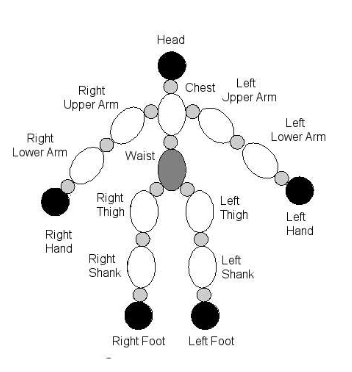
\includegraphics[scale=0.175]{images/humanoid-rigid-bodies.png}\hfill
    \caption{A rigid-body representation of humanoid robot}\hfill
    \label{humanoid-rigid-body}
\end{figure}

\subsection{ZMP}
\subsection{Dynamic Model of humanoid robot}
\subsection{Simplified dynamic model using LIPM}

\section{Control Approach}
\subsection{Balance Control}
\subsubsection{CoM tracking and scaling}
\subsubsection{ZMP tracking and scaling}

\subsection{Posture Control}
\subsubsection{Multi-Double Inverted Pendulum Model (M-DIP)}
\subsection{Acceleration Control}

\section{Task Specification Approach}

\subsection{Joint trajectory tracking}
\subsection{Balance Control}
\subsection{Posture Control}
\subsection{Joint Limits Avoidance}
